
\newpage
{\bfseries МРНТИ 20.15.13}

\sectionwithauthors{А.Тельман, Д.Р.Рашидинов, М. Тұрдалыұлы}{МОДЕЛИРОВАНИЕ ЦИФРОВЫХ БИЗНЕС-ПРОЦЕССОВ В ОБРАЗОВАТЕЛЬНЫХ
УЧРЕЖДЕНИЯХ}

\begin{center}


{\bfseries \textsuperscript{1}А.Тельман, \textsuperscript{1}Д.Р.Рашидинов\textsuperscript{🖂}, \textsuperscript{2, 3}М. Тұрдалыұлы}

\textsuperscript{1}Международный университет информационных технологий, г. Алматы,Казахстан,

\textsuperscript{2}Международный инженерно-технологический университет, г.Алматы, Казахстан,

\textsuperscript{3}Институт информационных и вычислительных технологий КН МНВО РК, Алматы, Казахстан,
\end{center}
Корреспондент-автор: \emph{damir.dmr88@gmail.com}\vspace{0.5cm}

Цифровизация затрагивает бизнес-процессы в сервисных организациях и
проявляется через внед-рение цифровых технологий для повышения их
эффективности. Это ведет к изменению бизнес-процессов и, в некоторых
случаях, к полной трансформации бизнес-модели компании. Экономисты и
специалисты прогнозируют, что такие изменения будут касаться всех
компаний в будущем.

Целью данного исследования является улучшение и внедрение методов
цифровизации бизнес-процессов в образовательных центрах для оптимизации
их работы, увеличения производительности и улучшения взаимодействия с
клиентами. В статье анализируется природа цифровизации в образова-нии и
рассматривается применение цифровизации в бизнес-процессах
образовательных учреждений.

В ходе исследования были выделены ключевые современные инструменты для
эффективного моде-лирования бизнес-процессов, которые помогают повысить
эффективность и конкурентоспособность бизнес-процессов, а также общую
производительность компании на фоне цифровизации. В рамках работы также
разработана методика оценки эффективности моделирования бизнес-процессов
в ус-ловиях цифровизации.

{\bfseries Ключевые слова:} цифровизация образования, цифровизация
процессов, улучшение процессов, образование, бизнес-процессы.

\sectionheading{БІЛІМ ОРЫНДАРЫНДАҒЫ ЦИФРЛЫҚ БИЗНЕС-ПРОЦЕСТЕРДІ МОДЕЛЬДЕУ}
\begin{center}

{\bfseries А.Тельман, Д.Р. Рашидинов\textsuperscript{🖂}б М. Тұрдалыұлы}

Халықаралық ақпараттық технологиялар университеті, Алматы, Қазақстан,

e-mail:damir.dmr88@gmail.com
\end{center}

Цифрландыру сервистік ұйымдардағы бизнес-процестерге әсер етеді және
олардың тиімділігін арттыру үшін цифрлық технологияларды енгізу арқылы
көрінеді. Бұл бизнес-процестердің өзгеруіне және кейбір жағдайларда
компанияның бизнес моделінің толық өзгеруіне әкеледі. Экономистер мен
сарапшылар мұндай өзгерістер болашақта барлық компанияларға әсер етеді
деп болжайды.

Бұл зерттеудің мақсаты -- білім беру орталықтарында олардың жұмысын
оңтайландыру, өнімділікті арттыру және клиенттермен өзара әрекеттесуді
жақсарту үшін бизнес-процестерді цифрландыру әдістерін жетілдіру және
енгізу. Мақалада білім берудегі цифрландырудың табиғаты талданып, білім
беру ұйымдарының бизнес-процестерінде цифрландыруды қолдану мәселелері
талқыланады.

Зерттеу бизнес-процестердің тиімділігі мен бәсекеге қабілеттілігін,
сондай-ақ цифрландыру аясын-да компанияның жалпы жұмысын жақсартуға
көмектесетін бизнес-процестерді тиімді модельдеудің негізгі заманауи
құралдарын анықтады. Жұмыс аясында цифрландыру жағдайында
бизнес-үдерістер-ді модельдеу тиімділігін бағалау әдістемесі де
әзірленді.

{\bfseries Түйін сөздер:} білім беруді цифрландыру, процестерді
цифрландыру, үдерістерді жетілдіру, білім беру, бизнес-процестер.

\sectionheading{MODELING DIGITAL BUSINESS PROCESSES IN EDUCATIONAL INSTITUTIONS}
\begin{center}

{\bfseries A.Telman, D.R.Rashidinov\textsuperscript{🖂}, M.Turdalyuly}

International University of Information Technologies, Almaty,
Kazakhstan,

e-mail:damir.dmr88@gmail.com
\end{center}

Digitalization affects business processes in service organizations and
manifests itself through the introduc-tion of digital technologies to
improve their efficiency. This leads to changes in business processes
and, in some cases, to a complete transformation of the
company\textquotesingle s business model. Economists and experts predict
that such changes will affect all companies in the future.

The purpose of this study is to improve and implement methods of
digitalization of business processes in educational centers to optimize
their work, increase productivity and improve interaction with
customers. The article analyzes the nature of digitalization in
education and considers the application of digitalization in the
business processes of educational institutions.

The study identified key modern tools for effective modeling of business
processes that help improve the efficiency and competitiveness of
business processes, as well as the overall performance of the company
against the background of digitalization. As part of the work, a
methodology for assessing the effectiveness of business process modeling
in the context of digitalization was also developed.

{\bfseries Key words:} digitalization of education, digitalization of
processes, process improvement, education, business processes.
\begin{multicols}{2}

{\bfseries Введение.} Современная цифровая революция разворачивается с
поразительной скоростью. Если переход от громоздких компьютеров к
персональным устройствам занял десятилетия, то новые технологические
модели могут меняться всего за несколько месяцев. Изначально
цифровизация охватывала автомати-зацию бизнес-процессов, улучшение
доступа в Интернет, развитие социальных сетей и внедрение новых
устройств, таких как планшеты и смартфоны. Сейчас, с ускорением
цифровизации, технологии становятся неотъем-лемой частью повседневной
жизни, включая сферу образования.

Цифровизация в образовании требует кардинальных изменений, так как
преподаватели должны адаптироваться к новым технологиям и эффективно их
использовать. Например, виртуальная реальность (VR) позволяет создавать
цифровые миры и симуляции, которые не подчиняются физическим
ограничениям. Это расширяет возможности обучения, а дистанционное
образование предоставляет доступ к образовательным ресурсам в любое
время и из любой точки мира.

Сегодня информация является краеугольным камнем глобального прогресса,
что делает традиционные подходы неадекватными. Как подчеркивает Л.В.
Шмелькова, важнейшей характеристикой людей, подходящих для цифровой
экономики, является их владение цифровыми технологиями и их применение в
профессиональной деятельности {[}1{]}.

Дети, которые приобрели навыки общения в цифровой среде за пределами
формального образования, особенно уязвимы перед последствиями оцифровки.

В то время как конкретным навыкам обучают на разных уровнях образования,
цифровые компетенции постоянно приобретаются и обновляются на протяжении
всей жизни. Таким образом, цифровизация образования тесно связана с
владением наставниками современными технологиями, поскольку им
необходимо эффективно внедрять их в образовательный процесс. Н.Н.
Битюцкая подчеркивает важность того, чтобы учителя приобрели навыки
ориентировки в потоке цифровой информации, умели работать с ней,
обрабатывать и интегрировать в новые технологии {[}2{]}. Система
цифрового образования состоит из таких элементов, как: информационные
ресурсы, телекоммуникации и управляющая система (рис. 1).
\end{multicols}

\begin{figure}[H]
	\centering
	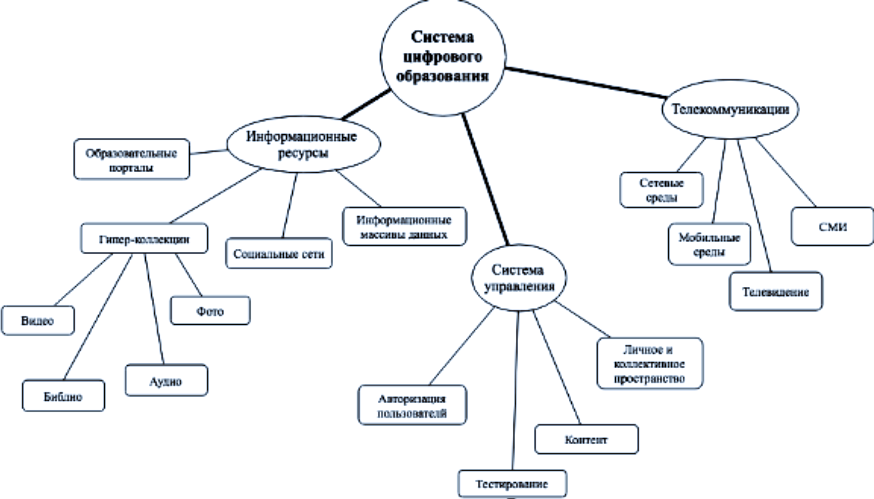
\includegraphics[width=0.8\textwidth]{assets/205.1}
	\caption*{\bfseries Рис. 1 -- Составляющие системы цифрового образования}
\end{figure}


\begin{multicols}{2}

{\bfseries Материалы и методы.} Использование новых технологий, механизмов
и алгоритмов в образовательном процессе требует их эффективного
использования. Дистанционное и смешанное обучение предоставляют людям
огромные возможности для доступа к качественному образованию, независимо
от их географического положения и имеющихся навыков, а также с учетом их
конкретных требований и возможностей.

Эти изменения требуют, чтобы учителя обладали всесторонним пониманием
цифровой сферы. Поэтому крайне важно установить "единые стандарты для
уже существующих и разрабатываемых онлайн-курсовых платформ, чтобы они
могли быть интегрированы в единую систему, аналогичную "единому окну".

Условия для оцифровки можно сформулиро-вать следующим образом:

1. всеобщий доступ: физические лица и организации на всей территории
Казахстана, независимо от их местонахождения, должны иметь доступ к
информационным ресурсам и возможностям, необходимым для их личной и
деловой деятельности, бесплатно или за плату

2. доступность технологий: общество должно обеспечить свободный доступ к
соответствующим цифровым технологиям и обеспечить практическую
реализацию вышеуказанных условий

3. развитие инфраструктуры: должна быть создана достаточная
инфраструктура для поддержки национальных информационных ресурсов,
необходимых для развития быстро эволюционирующего общества. Общество
должно генерировать и хранить всю информацию, необходимую для его
функционирования, в частности научные знания.

4. автоматизация: должна происходить непрерывная автоматизация всех сфер
экономической и социальной жизни общества.

5. глобальное влияние: расширение цифровой деятельности и
информационно-коммуникацион-ных услуг происходит под влиянием глобальной
трансформации социальных структур.

В последнее время разработка и использование открытых онлайн-ресурсов
набрали значительный импульс. Это включает в себя целый ряд ресурсов, от
индивидуальных заданий и тестов до комплексных курсов и модулей,
направленных на формирование необходимых компетенций. Растущая
доступность онлайн-курсов свидетельствует о динамичном развитии
онлайн-обучения.

Цифровизация образования выходит за рамки онлайн-курсов и включает в
себя развитие цифровых библиотек и виртуальных университетских городков.
Создание и внедрение онлайн-курсов предполагает использование
программных решений, которые позволяют собирать курсы из существующих
информационных ресурсов и специализированных программных сред.

Образование играет решающую роль в развитии интеллекта людей и
обеспечении их возможности трудоустройства в эпоху цифровых
преобразований. Это считается одним из основных принципов, с помощью
которых развиваются и совершенствуются навыки сотрудников. Осваивая
цифровизацию, школьники и студенты могут получить более глубокое
представление о реальном мире, особенно о современных технологиях
{[}3{]}.

Исследования показывают, что уже 37 процентов образовательных
организаций по всему миру применяют искусственный интеллект, включая
чат-ботов, для учебного процесса {[}4{]}. Студенты и ученики высоко
оценивают взаимодействие с программой и считают, что она способствует
лучшему обучению, по сравнению с человеком. Теперь давайте разберемся,
что представляют собой чат-боты и почему они востребованы в образовании.

На основании исследования использования чат-ботов в образовательном
процессе, можно выделить следующие рекомендации для повышения их
эффективности:

\begin{enumerate}
\def\labelenumi{\arabic{enumi}.}
\setlength{\itemindent}{1cm}
\item
  Преимущества использования Telegram-ботов в образовании:

  \begin{itemize}
    \setlength{\itemindent}{1cm}
  \item
    Быстрая коммуникация между студента-ми и преподавателями.
  \item
    Участие и вовлеченность в образователь-ный процесс.
  \item
    Удобное хранение материалов курса и работ студентов.
  \item
    Отсутствие необходимости загружать дополнительные приложения.
  \item
    Бесплатное использование.
  \end{itemize}
\item
  Недостатки использования Telegram-ботов в образовании:

  \begin{itemize}
    \setlength{\itemindent}{1cm}
  \item
    Возможное увеличение нагрузки на преподавателя.
  \item
    Отвлечение студентов от основных тем обсуждения или взаимодействие с
    другими участниками чата.
  \item
    Необходимость наличия смартфона с доступом в интернет.
  \item
    Возможная потеря информации, хранящейся на мобильных устройствах.
  \end{itemize}
\item
  Чат-боты в образовании должны быть простыми, быстрыми в поиске
  информации и обеспечивать безопасный доступ к ней. Их интерфейс должен
  быть понятным и удобным для пользователей. Такие инструменты
  коммуникации помогут ускорить и упростить взаимодействие между
  студентами и преподавателями, экономя время.
\item
  Чат-боты могут использоваться для проведения тематических
  онлайн-квестов, предоставления нового материала и развития
  коммуникации между преподавателями и студентами. Они также могут
  способствовать вовлечению студентов в новые формы обучения и
  познавательной деятельности.
\end{enumerate}

Одним из основных преимуществ чат-ботов является их широкая
популярность. Отправка сообщений через мессенджеры удобна и не создает
дополнительной нагрузки на приложение. Коммуникация в чат-ботах краткая,
информативная и быстрая. Благодаря этому педагоги могут быстро и легко
устанавливать контакт с учениками и своевременно передавать им всю
важную информацию {[}5{]}.

Эффективность взаимодействия и коммуника-ции между преподавателями и
учениками, адаптация к изменяющимся условиям и успешное внедрение новых
технологий в образовательный процесс влияют на развитие системы
образования и государства в целом {[}6{]}.

{\bfseries Обсуждение и результаты.} При цифровиза-ции бизнес-процессов и
внедрении чат-бота в организацию необходимо оценить их эффективность и
целесообразность. Для этого можно использовать язык моделирования
бизнес-процессов BPMN (Business Process Model and Notation), который
поможет описать и визуализировать процессы и их реализацию в различных
системах управления.

BPMN является составной частью двух основных компонентов:

- BPM (бизнес-процессное моделирование) - это среда, в которой вы
активно участвуете в создании моделей, как в одиночку, так и в команде.

-BPMS (система моделирования бизнес-процессов) - это инструменты,
которые позволяют выполнить созданные вами модели. Примерами таких
инструментов являются Bizagi, Comundo, ELMA и другие.

Создание BPMN-диаграммы для образователь-ного центра требует знаний в
области бизнес-анализа; BPMN-модель не ограничивается простыми
картинками и диаграммами, которые можно нарисовать в графическом
редакторе. Важным аспектом является правильная структура и
последовательность процессов.

Чтобы показать, как принципы бизнес-моделирования реализуются в
событийно-процессной нотации, рассмотрим пример процесса, который входит
в контракт курса бизнес-анализа в современной образовательной школе.

\begin{enumerate}
\def\labelenumi{\arabic{enumi}.}
\setlength{\itemindent}{1cm}
\item
  Процесс начинается с того, что заказчик оставляет заявку на сайте.
\item
  На основании заявки менеджер формирует коммерческое предложение,
  которое, в зависимости от предоставленных контактных данных,
  озвучивается по телефону или отправляется на электронную почту
  клиента.
\item
  Клиент принимает решение на основании предложения. Если клиент не
  желает проходить обучение, процесс работы с ним завершается.
\item
  Если клиент согласен с условиями, он сообщает менеджеру о своем
  намерении заключить договор и предоставляет необходи-мые данные.
\item
  Менеджер готовит проект договора и отправляет его клиенту на
  согласование.
\item
  Если у клиента нет возражений, договор подписывается, и процесс
  заключения договора завершается. Начинается процесс оплаты, который
  описан на другой схеме.
\item
  Если по проекту договора есть возражения, клиент вносит изменения и
  отправляет его менеджеру.
\end{enumerate}

Менеджер готовит новый проект договора и отправляет его обратно клиенту
на утверждение, повторяя шаги 5-7.

Чтобы улучшить понимание диаграммы, мы разделили процесс на две части:
обработку заявки и заключение договора. Клиента представляем внешним
закрытым пулом, с которым взаимодействуем через потоки сообщений. Для
компактного размещения элементов диаграммы мы предусмотрели обход потока
сообщений между пулами, чтобы избежать пересечений линий и упростить
диаграмму (рис. 2).
\end{multicols}

\begin{figure}[H]
	\centering
	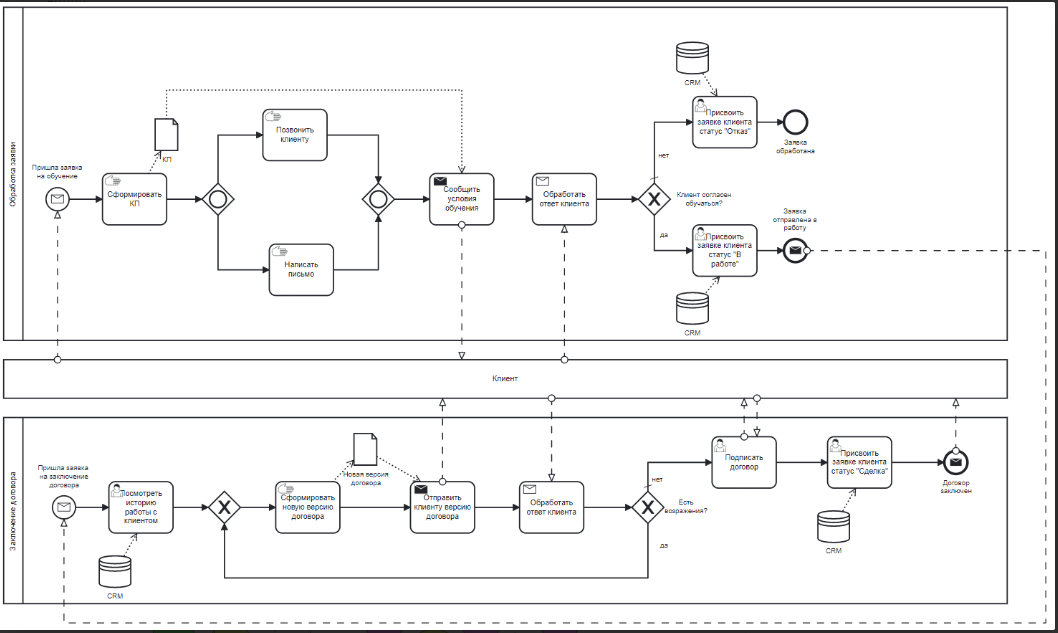
\includegraphics[width=0.7\textwidth]{assets/206}
	\caption*{\bfseries Рис. 2 -- BPMN-диаграмма для образовательного центра}
\end{figure}


\begin{multicols}{2}

В ходе работы был разработан соответствующий алгоритм (рис.3) для оценки
эффективности моделирования бизнес-процессов компании в условиях
цифровизации. Этот алгоритм представляет собой подробную схему с
определенными вариантами исполнения этапов и принимаемых решений,
включая как положительные, так и отрицательные их развития. Все это
отображено в графическом виде.
\end{multicols}

\begin{figure}[H]
	\centering
	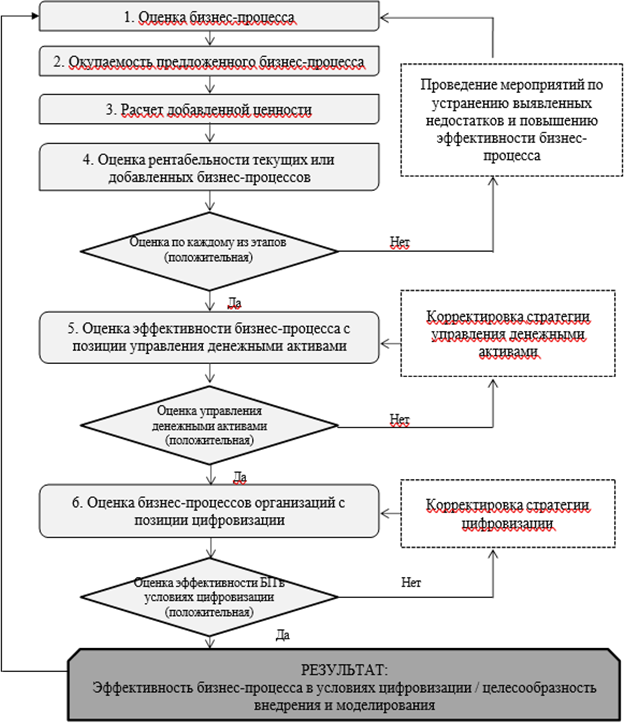
\includegraphics[width=0.5\textwidth]{assets/207}
	\caption*{\bfseries Рис. 3 -- Алгоритм оценки эффективности моделирования бизнес-
  процессов компании в условиях цифровизации}
\end{figure}

\begin{multicols}{2}


Алгоритм оценки эффективности моделирова-ния бизнес-процессов компании в
условиях цифровизации, начинается с исследования бизнес-процесса, его
организации, степени выполнения, в том числе общей оценки. Следующим
этапом в предложенной методике является оценка окупаемости предложенного
бизнес-процесса. Данный этап является расчетным, расчет окупаемости
предложенного бизнес-процесса осуществляется по формуле (1):


\begin{equation}
  \text{ПО} = \text{ИС} / \text{ДПn}
\end{equation}

где ПО -- период окупаемости предложенного бизнес-процесса;

ИС -- сумма инвестиционных средств, которые направлены на реализацию
предлагаемого бизнес-процесса, тыс.тг.;

ДПn -- средняя сумма денежного потока от реализации предлагаемого
бизнес-процесса, (заработная плата одного оператора) тыс.тг.;

n -- количество периодов, в данном случае 1.

ПО = 1600 / 170 *12 = 0,76 года = 8 мес.

Характеризуя вышеуказанный показатель, следует обратить внимание на то,
что он может быть использован для оценки не только эффективности
предлагаемого бизнес-процесса, но и уровня рисков.

Последующим этапом в алгоритме оценки эффективности моделирования
бизнес-процессов компании в условиях цифровизации является расчет
добавленной стоимости.

Добавленная ценность служит теоретической концепцией, которая выражает
соотношение рыночной стоимости и фактически понесенных затрат от
предлагаемого бизнес-процесса. Величину добавленной ценности (AV) можно
рассчитать по формуле (2):

\begin{equation}
  \text{AV} = \text{Va - Vb }
\end{equation}
 

Va -- ценность бизнес-процесса после обработки;

Vb -- ценность бизнес-процесса перед обработкой.

\begin{center}
AV = 3~656~000 -- 3~000~000 = 656 тыс. тг
\end{center}


С целью оценки эффективности моделирования бизнес-процессов, которые
добавляют экономичес-кую ценность (затраты), на отдельном бизнес-
процессе данную ценность можно выразить в виде определенного удельного
показателя.

Оценка рентабельности текущих или добавленных бизнес-процессов --
следующий этап в разработанном алгоритме оценки эффективности
моделирования бизнес-процессов компании в условиях цифровизации. Данный
показатель является относительным уровнем прибыльности от предлагаемого
бизнес-процесса в компании.

Рентабельность текущих или добавленных бизнес-процессов (Р)
рассчитывается по формуле (3):

\begin{equation}
\text{P = П / В}
\end{equation}

П -- прибыль от текущих или добавленных бизнес-процессов в организации,
тыс.тг.;

В -- выручка от текущих или добавленных бизнес-процессов в организации,
тыс.тг..
\begin{center}
P = 1200 / 2450 =0,49 = 49\%
\end{center}


В условиях получения оптимального значения (более 4\%), повышения его в
динамике (в сравнении с текущим показателем, то есть показателем
отчетного периода), необходимо перейти к следующему этапу в
разработанной методике. В условиях значения до 4\%, сокращения его в
динамике, следует проводить мероприятия по устранению выявленных
недостатков и повышению эффективности моделирования бизнес-процесса в
компании, чтобы впоследствии вернуться к этапу и перейти к последующему
по разработанной методике {[}7{]}.

Оценка эффективности бизнес-процесса с позиции управления денежными
активами -- пятый этап в алгоритме оценки эффективности моделирования
бизнес-процессов компании в условиях цифровизации. На данном этапе
проводится расчет по основным показателям эффективности: степени участия
денежных активов бизнес-процессов в совокупных оборотных активах
организации, среднему периоду оборота и количества оборотов денежных
активов бизнес-процессов в рассматриваемом периоде, количеству оборотов
среднего остатка денежных активов в рассматриваемом периоде для бизнес-
процессов, коэффициенту рентабельности краткосрочных финансовых
инвестиций для бизнес-процессов, а также планируемой суммы операционного
остатка денежных активов бизнес-процессов (табл. 1).
\end{multicols}
{\bfseries Таблица 1 -- Показатели эффективности моделирования
бизнес-процесса с позиции \\управления денежными активами}\vspace{0.5cm}
\begin{longtable}[]{|@{}
  >{\raggedright\arraybackslash}p{(\columnwidth - 4\tabcolsep) * \real{0.2722}}|
  >{\raggedright\arraybackslash}p{(\columnwidth - 4\tabcolsep) * \real{0.3070}}|
  >{\raggedright\arraybackslash}p{(\columnwidth - 4\tabcolsep) * \real{0.4207}}@{}|}
\hline
\toprule\noalign{}
\begin{minipage}[b]{\linewidth}\raggedright
Наименование показателя
\end{minipage} & \begin{minipage}[b]{\linewidth}\raggedright
Сущность показателя
\end{minipage} & \begin{minipage}[b]{\linewidth}\raggedright
Расчет (формула с пояснениями)
\end{minipage} \\
\hline
\midrule\noalign{}
\endfirsthead
\hline
\toprule\noalign{}
\begin{minipage}[b]{\linewidth}\raggedright
Наименование показателя
\end{minipage} & \begin{minipage}[b]{\linewidth}\raggedright
Сущность показателя
\end{minipage} & \begin{minipage}[b]{\linewidth}\raggedright
Расчет (формула с пояснениями)
\end{minipage} \\
\hline
\endhead
\hline
\bottomrule\noalign{}
\endlastfoot
Степень участия денежных активов бизнес-процессов в совокупных оборотных активов организации (КУ) & Показывает степень участия денежных активов предприятия в оборотном капитале в условиях реализации бизнес-процессов & {\bfseries КУ = ДА / ОА}

ДА -- средний остаток совокупных денежных активов, тыс.тг.;

ОА -- средняя сумма оборотных активов организации, тыс.тг. \\
\hline
Средний период оборота и количество оборотов денежных активов бизнес-процессов в рассматриваемом периоде (ПО) & Показывает степень оборачиваемости активов в условиях реализации бизнес- процессов & {\bfseries пО = ДА / РДА}

РДА -- однодневный объем расходования денежных средств, тыс.тг. \\
\hline
Количество оборотов среднего остатка денежных активов в рассматриваемом периоде для бизнес- процессов (КО) & Показывает степень оборачиваемости среднего остатка денежных активов & {\bfseries КО = РДАо / ДА}

РДАо -- общий объем расходования денежных средств, тыс.тг. \\
\hline
Коэффициент рентабельности краткосрочных финансовых инвестиций для бизнес-процессов (КРкфи) & Показывает степень прибыльности краткосрочных финансовых инвестиций для бизнес-процессов, то есть экономическую целесообразность их ввода & {\bfseries КРкфи = П / КФИ}

П -- сумма прибыли, которая получена организацией от инвестирования, тыс.тг. \\
\hline
Планируемая сумма операционного остатка денежных активов бизнес-процессов (Дао) & Показывает потребность в остатках денежных активов бизнес-процессов в условиях реализации бизнес-процессов & {\bfseries ДАо = пО / КО}

пО -- планируемый объем отрицательного денежного потока, тыс.тг.;

КО -- количество оборотов среднего остатка денежных активов по плану. \\
\hline
\end{longtable}

\begin{multicols}{2}

Также как и было указано ранее, при положительной оценке бизнес-
процесса с позиции управления денежными активами (приросте в динамике,
например в сравнении с отчетными показателями), выполняется следующий
этап, а при сокращении, небольших значениях -- происходит корректировка
существующей или выбранной стратегии управления денежными активами в
компании, чтобы также вернуться к данному этапу, достичь запланированных
целей и задач.

{\bfseries Выводы.} Существует множество подходов и принципов для
модернизации образовательного процесса. Одним из ключевых аспектов
является мотивация и заинтересованность учеников. Быстрые
технологические изменения существенно изменили ожидания детей от
учебного процесса. Традиционные методы уже не вызывают у них интерес,
поэтому педагогам необходимо адаптироваться к современным требованиям и
искать новые подходы в обучении.

Эта тенденция вынуждает учителей искать инновационные методы работы,
что, в свою очередь, предоставляет им возможность развиваться, улучшать
свои педагогические навыки и открывает новые горизонты для преподавания.
Правильно подобранные методы обучения помогают учителям завоевать
уважение учеников и поддерживать их интерес к учебе.

Быстрые изменения в обществе требуют оперативной адаптации методов
преподавания. Чем быстрее учителя осваивают новые возможности и
учитывают потребности учеников, тем более эффективным становится
образовательный процесс. Качество знаний, полученных в школе, напрямую
влияет на уровень квалификации будущих специалистов в различных
областях.

Цель данной работы заключалась в разработке и внедрении методов
цифровизации для бизнес-процессов в образовательных центрах. Это
позволит оптимизировать множество бизнес-процессов, повысить
производительность и улучшить взаимодействие с клиентами.

Анализ показал особенности моделирования бизнес-процессов в условиях
цифровизации, такие как расширение функций специалистов, использование
различных цифровых инструмен-тов и технологий, а также автоматизация
процессов.

На основе исследования была разработана методика моделирования
бизнес-процессов с учетом цифровизации. Эта методика представляет собой
универсальный подход к изучению и оценке процессов, включающий
соответствующие факторы и инструменты для достижения целей, создания
конкурентной среды на рынке, соответствия мировым стандартам и улучшения
качества в условиях современных потребительских тенденций.

\end{multicols}

\begin{center}
  {\bfseries Литература}
  \end{center}

\begin{noparindent}

1.Козлов С.В., Резванцева А.А. Чат-боты как одна из тенденций развития
современного образования // Международный журнал экспериментального
образования.-2022.-№ 5. - С. 44-49.
\\https://expeducation.ru/ru/article/view?id=12095~

2.Грекул В.И., Денищенко Г.Н., Коровкина Н.Л. Управление внедрением
информационных систем. Методология внедрения OneMethodology. -512 с.
2021 г., издание, ISBN 978-5-4497-0910-3

3.Антонов, Г.Д. Управление проектами организации: учебник / Г.Д.
Антонов, О.П. Иванова, В.М. Тумин. -- Москва: Инфра-М, 2018.- 244 c.
ISBN 978-5-16-01332-0

4.Гузь, Д.А. Улучшение конкурентоспособности предприятия с помощью
моделирования бизнес-процессов / Д.А. Гузь, Ю.С. Бровкова // Концепции и
модели устойчивого инновационного развития общества: сборник статей
международной научно-практической конференции. -- Омега Сайнс, 2020. -
С. 52-56.

5.Буленко, Ю.А. Структурная модель развития бизнес-процессов компании /
Ю.А. Буленко // Мате-риалы и методы инновационных исследований и
разработок: сборник статей международной научно-практической
конференции. -- Омега Сайнс, 2019. -- С. 96-97.

6.Ктет М.А. Оценка факторов, влияющих на поведение потребителей
гостиничных услуг //диссерта-ция кандидата экономических наук.-
Владивосток, 2020. -- 230 с.

7.Смыслова Л.В. Чат-бот как современное средство интернет- коммуникаций
// Молодой ученый. - 2018. - № 9. - С. 36-39
\end{noparindent}

\begin{center}
  {\bfseries References}
  \end{center}

\begin{noparindent}

1.Kozlov S.V., Rezvanceva A.A. Chat-boty kak odna iz tendencij razvitija
sovremennogo obrazovanija // Mezhdunarodnyj zhurnal
jeksperimental\textquotesingle nogo obrazovanija.-2022.-№ 5. - S. 44-49.
\\https://expeducation.ru/ru/article/view?id=12095

2.Grekul V.I., Denishhenko G.N., Korovkina N.L. Upravlenie vnedreniem
informacionnyh sistem. Meto-dologija vnedrenija OneMethodology. -512 s.
2021. ISBN 978-5-4497-0910-3

3.Antonov, G.D. Upravlenie proektami organizacii: uchebnik / G.D.
Antonov, O.P. Ivanova, V.M. Tumin. -- Moskva: Infra-M, 2018.- 244 c.
ISBN 978-5-16-01332-0

4.Guz\textquotesingle, D.A. Uluchshenie konkurentosposobnosti
predprijatija s pomoshh\textquotesingle ju modelirovanija
biznes-proces-sov / D.A. Guz\textquotesingle, Ju.S. Brovkova // Koncepcii
i modeli ustojchivogo innovacionnogo razvitija obshhestva: sbornik
statej mezhdunarodnoj nauchno-prakticheskoj konferencii. -- Omega Sajns,
2020. - S. 52-56.

5.Bulenko, Ju.A. Strukturnaja model\textquotesingle{} razvitija
biznes-processov kompanii / Ju.A. Bulenko // Materialy i metody
innovacionnyh issledovanij i razrabotok: sbornik statej mezhdunarodnoj
nauchno-prakticheskoj konferencii. -- Omega Sajns, 2019. -- S. 96-97.

6.Ktet M.A. Assessment of factors influencing the behavior of consumers
of hotel services // dissertation of candidate of economic sciences. -
Vladivostok, 2020. - 230 p.

7.Smyslova L.V. Chat-bot kak sovremennoe sredstvo internet- kommunikacij
// Molodoj uchenyj. - 2018. - № 9. - S. 36-39
\end{noparindent}

\emph{{\bfseries Сведения об авторах}}
\begin{noparindent}

Тельман А. Б. - магистр, Международный университет информационных
технологий, г. Алматы, Казахстан, e-mail: telmanalisher@gmail.com

Рашидинов Д.Р. -докторант, Международный университет информационных
технологий, г. Алматы, Казахстан, e-mail: damir.dmr88@gmail.com

М. Тұрдалыұлы- PhD, ассоциированный профессор, Международный инженерно-технологический
университет,Институт информационных и вычислительных технологий КН МНВО РК, \\e-mail:m.turdalyuly@gmail.com
\end{noparindent}

\emph{{\bfseries Information about the authors}}
\begin{noparindent}

Telman A.B.- Master, International University of Information
Technologies, Almaty, Kazakhstan,\\ e-mail: telmanalisher@gmail.com

Rashidinov D. R. - Doctoral student, International University of
Information Technologies, Almaty,\\ Kazakhstan, e-mail:
damir.dmr88@gmail.com

Turdalyuly M. - PhD, Associate Professor, International engineering and Technology University, RSE Institute of
Information and Computational Technologies MSHE RK CS, Almaty, Kazakhstan, e-mail: m.turdalyuly@gmail.com
\end{noparindent}









